\documentclass[letterpaper, 11pt]{extarticle}

% ==================================================
% document parameters
\usepackage[english]{babel}
\usepackage[margin=1in]{geometry}

% ==================================================
% Packages for math
\usepackage{mathrsfs}
\usepackage{amsfonts}
\usepackage{amsmath}
\usepackage{amsthm}
\usepackage{amssymb}
\usepackage{physics}
\usepackage{dsfont}
\usepackage{esint}
\usepackage{tikz}
\usepackage{url}
\usepackage[framed,numbered,autolinebreaks,useliterate]{mcode}

% ==================================================
% Packages for writing
\usepackage{enumerate}
\usepackage[shortlabels]{enumitem}
\usepackage{framed}
\usepackage{csquotes}

% ==================================================
% Miscellaneous packages
\usepackage{float}
\usepackage{tabularx}
\usepackage{xcolor}
\usepackage{multicol}
\usepackage{subcaption}
\usepackage{caption}
\captionsetup{format=hang, margin=10pt, font=small, labelfont=bf}

% Citation
\usepackage[round, authoryear]{natbib}

% Hyperlinks setup
\usepackage{hyperref}
\definecolor{links}{rgb}{0.36,0.54,0.66}
\hypersetup{
   colorlinks=true,
    linkcolor=black,
     urlcolor=blue,
    citecolor=blue,
    filecolor=blue,
    pdfauthor={Author},
     pdftitle={Title},
   pdfsubject={subject},
  pdfkeywords={one, two},
  pdfproducer={LaTeX},
   pdfcreator={pdfLaTeX},
}
\usepackage{titlesec}
\usepackage[many]{tcolorbox}

% Adjust spacing after the chapter title
\titlespacing*{\chapter}{0cm}{-2.0cm}{0.50cm}
\titlespacing*{\section}{0cm}{0.50cm}{0.25cm}

% Indent 
\setlength{\parindent}{0pt}
\setlength{\parskip}{1ex}

% --- Theorems, lemma, corollary, postulate, definition ---
% \numberwithin{equation}{section}

\newtcbtheorem[]{problem}{Problem}%
    {enhanced,
    colback = black!5, %white,
    colbacktitle = black!5,
    coltitle = black,
    boxrule = 0pt,
    frame hidden,
    borderline west = {0.5mm}{0.0mm}{black},
    fonttitle = \bfseries\sffamily,
    breakable,
    before skip = 3ex,
    after skip = 3ex
}{problem}

\tcbuselibrary{skins, breakable}

% --- You can define your own color box. Just copy the previous \newtcbtheorm definition and use the colors of yout liking and the title you want to use.
% --- Basic commands ---
%   Euler's constant
\newcommand{\eu}{\mathrm{e}}

%   Imaginary unit
\newcommand{\im}{\mathrm{i}}

%   Sexagesimal degree symbol
\newcommand{\grado}{\,^{\circ}}

% --- Comandos para álgebra lineal ---
% Matrix transpose
\newcommand{\transpose}[1]{{#1}^{\mathsf{T}}}

%%% Comandos para cálculo
%   Definite integral from -\infty to +\infty
\newcommand{\Int}{\int\limits_{-\infty}^{\infty}}

%   Indefinite integral
\newcommand{\rint}[2]{\int{#1}\dd{#2}}

%  Definite integral
\newcommand{\Rint}[4]{\int\limits_{#1}^{#2}{#3}\dd{#4}}

%   Dot product symbol (use the command \bigcdot)
\makeatletter
\newcommand*\bigcdot{\mathpalette\bigcdot@{.5}}
\newcommand*\bigcdot@[2]{\mathbin{\vcenter{\hbox{\scalebox{#2}{$\m@th#1\bullet$}}}}}
\makeatother

%   Hamiltonian
\newcommand{\Ham}{\hat{\mathcal{H}}}

%   Trace
\renewcommand{\Tr}{\mathrm{Tr}}

% Christoffel symbol of the second kind
\newcommand{\christoffelsecond}[4]{\dfrac{1}{2}g^{#3 #4}(\partial_{#1} g_{#2 #4} + \partial_{#2} g_{#1 #4} - \partial_{#4} g_{#1 #2})}

% Riemann curvature tensor
\newcommand{\riemanncurvature}[5]{\partial_{#3} \Gamma_{#4 #2}^{#1} - \partial_{#4} \Gamma_{#3 #2}^{#1} + \Gamma_{#3 #5}^{#1} \Gamma_{#4 #2}^{#5} - \Gamma_{#4 #5}^{#1} \Gamma_{#3 #2}^{#5}}

% Covariant Riemann curvature tensor
\newcommand{\covariantriemanncurvature}[5]{g_{#1 #5} R^{#5}{}_{#2 #3 #4}}

% Ricci tensor
\newcommand{\riccitensor}[5]{g_{#1 #5} R^{#5}{}_{#2 #3 #4}}

\documentclass{article}
\usepackage[framed,numbered,autolinebreaks,useliterate]{mcode}  % For MATLAB code
\usepackage{graphicx} % For logos
\usepackage{tikz} % For custom graphics
\usepackage{fancyhdr} % For header and footer customization

\begin{document}

% Title Page
\begin{titlepage}
    \begin{center}
        % School Logo
        
\includegraphics[width=0.3\textwidth]{ENSI.png} \\  
        \vspace{1cm}
        
        % Project Title
        {\Huge \textbf{Compte Rendu }} \\
        \textbf{TP1: Mise à niveau pour l’exploitation des boîtes à outils de Matlab
Toolbox Matlab, control et Simulink. }} \\
        \vspace{1cm}
        
        % Project Logo
        
\includegraphics[width=0.6\textwidth]{Matlab_Logo.png} \\
        \vspace{2cm}

        % Étudiants Names
        \textbf{\Large \textsf{Étudiants:}} \\
        \textsf{Taha Taidi Laamiri} \\
        \textsf{Achraf Amziane} \\
        \textsf{Mohamed BELKHIR} \\
       
        \vspace{0.5cm}
        
        % Teacher Name
        \textbf{\Large \textsf{Professeur:}} \\
        \textsf{Marouane ANCARI} \\
        \vspace{1cm}

        % Date
        {\large \textsf{\today}}
        
        \vfill
        \textit{\footnotesize Note: Ce document a été rédigé en utilisant \LaTeX.}
    \end{center}
\end{titlepage}



% Main Content
\begin{Large}
    \textsf{\textbf{Rapport d'Exercice}}
    
    \vspace{1ex}
\end{Large}

\vspace{2ex}

\textsf{\textbf{Exercice 1 :}}
\begin{problem}{Tracer une fonction sinuso\"idale}{exercise-label-1}
Soit la fonction suivante :
\[ y = \sin(t), \quad t : \text{le temps.} \]
\`Ecrire un programme sous \texttt{Matlab} pour tracer cette fonction pour \( 0 \leq t \leq 2\pi \) avec un pas de \( \pi/100 \) et en indiquant sur la figure :
\begin{itemize}
    \item \textbf{Le titre :} Fonction sinuso\"idale,
    \item \textbf{L'axe \( X \) :} Temps en secondes (s),
    \item \textbf{L'axe \( Y \) :} Amplitude.
\end{itemize}
Mettre la grille sur la figure.
\end{problem}

\textsf{\textbf{Solution :}}

\subsection*{Programme MATLAB :}
\begin{lstlisting}
% Define the time range
t = 0:pi/100:2*pi;               

% Compute the sine function
y = sin(t);                      

% Plot the function
plot(t, y);                      
\end{lstlisting}

\textsf{\textbf{Graph avec grille :}}


\begin{center}
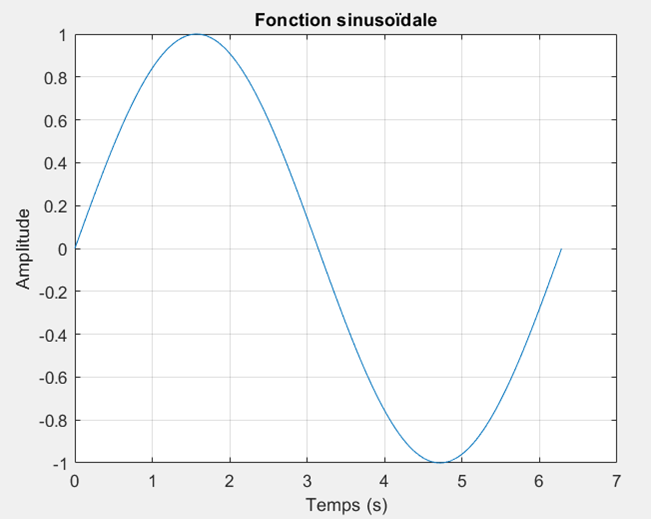
\includegraphics[width=0.5\textwidth]{EXERCICE 1 GRAPH.png}
\end{center}

\newpage

\textsf{\textbf{Exercice 2 :}}
\begin{problem}{Calculs sur une fonction polynomiale}{exercise-label-2}
Ecrire l'\'equation suivante sous \texttt{Matlab} :
\[ y(t) = 5t^4 + 5t^2 + 8t - 1, \quad t : \text{\'etant le temps.} \]
\begin{itemize}
    \item Calculer les racines de \( y(t) \),
    \item Calculer \( y(-1) \), \( y(1) \), \( y(2) \),
    \item Calculer \( \frac{dy(t)}{dt} \),
    \item Calculer \( z(t) = y(t) \cdot x(t) \) avec \( x(t) = 9t^2 + t + 5 \).
\end{itemize}
\end{problem}

\textsf{\textbf{Solution :}}

\subsection*{Question 1}
\textbf{Écrire l'équation suivante sous MATLAB :}  
\( y(t) = 5t^4 + 5t^2 + 8t - 1 \), \( t \) étant le temps.

\subsection*{Programme MATLAB :}
\begin{lstlisting}[language=Matlab]
syms t
y = 5*t^4 + 5*t^2 + 8*t - 1;
\end{lstlisting}

\subsection*{Question 2}
\textbf{Calculer les racines de \( y(t) \).}

\subsection*{Programme MATLAB :}
\begin{lstlisting}[language=Matlab]
% Calcul des racines de y(t)
racines = solve(y == 0, t);
disp('Racines de Y(t) :');
disp(racines);
\end{lstlisting}

\textbf{Résultats :}
\begin{verbatim}
Racines de Y(t) :
root(z^4 + z^2 + (8*z)/5 - 1/5, z, 1)
root(z^4 + z^2 + (8*z)/5 - 1/5, z, 2)
root(z^4 + z^2 + (8*z)/5 - 1/5, z, 3)
root(z^4 + z^2 + (8*z)/5 - 1/5, z, 4)
\end{verbatim}

\newpage
\subsection*{Question 3}
\textbf{Calculer \( y(-1) \), \( y(1) \), \( y(2) \).}

\subsection*{Programme MATLAB :}
\begin{lstlisting}[language=Matlab]
disp('Valeurs de Y(t) :');
disp(['Y(-1) = ', char(subs(y, t, -1))]);
disp(['Y(1) = ', char(subs(y, t, 1))]);
disp(['Y(2) = ', char(subs(y, t, 2))]);
\end{lstlisting}

\textbf{Résultats :}
\begin{verbatim}
Valeurs de Y(t) :
Y(-1) = 1
Y(1) = 17
Y(2) = 115
\end{verbatim}

\subsection*{Question 4}
\textbf{Calculer \( \frac{dy(t)}{dt} \).}

\subsection*{Programme MATLAB :}
\begin{lstlisting}[language=Matlab]
% Calcul de la dérivée DY(t)/DT
dy = diff(y, t);
disp('Dérivée DY(t)/DT :');
disp(dy);
\end{lstlisting}

\textbf{Résultat :}
\begin{verbatim}
Dérivée DY(t)/DT :
20*t^3 + 10*t + 8
\end{verbatim}

\newpage
\subsection*{Question 5}
\textbf{Calculer \( z(t) = y(t) \cdot x(t) \) avec \( x(t) = 9t^2 + t + 5 \).}

\subsection*{Programme MATLAB :}
\begin{lstlisting}[language=Matlab]
% Définition de X(t)
x = 9*t^2 + t + 5;

% Calcul de Z(t) = Y(t) * X(t)
z = y * x;
disp('Fonction Z(t) :');
disp(z);
\end{lstlisting}

\textbf{Résultats :}
\begin{verbatim}
Fonction Z(t) :
(9*t^2 + t + 5)*(5*t^4 + 5*t^2 + 8*t - 1)
\end{verbatim}


\newpage

\textsf{\textbf{Exercice 3 :}}
\begin{problem}{Fonctions de transfert sous Matlab}{exercise-label-3}
\'Ecrire sous \texttt{Matlab}, les fonctions de transfert suivantes selon deux m\'ethodes :
\[
F_1(p) = \frac{1}{p+6}, \quad
F_2(p) = \frac{p+2}{p(p-5)}, \quad
F_3(p) = \frac{7(p+9)}{p^2 + 2p + 5}, \quad
F_4(p) = \frac{5(p-7)}{p^2 + 0.99p + 0.4}.
\]
\end{problem}

\textsf{\textbf{Solution :}}

\subsection*{Fonction $F_1(p) = \frac{1}{p + 6}$}

\subsubsection*{Méthode 1 : Utilisation de \texttt{tf}}
\subsection*{Programme MATLAB :}
\begin{lstlisting}[language=Matlab]
% F1(p) = 1 / (p + 6)
num1 = 1; 
den1 = [1 6]; 
F1_tf = tf(num1, den1);
\end{lstlisting}

\textbf{Résultat :}
\begin{verbatim}
F1_tf =
    1
  -----
  s + 6
Continuous-time transfer function.
\end{verbatim}

\subsubsection*{Méthode 2 : Utilisation de \texttt{zpk}}
\subsection*{Programme MATLAB :}
\begin{lstlisting}[language=Matlab]
% F1(p)
z1 = []; 
p1 = -6; 
k1 = 1;
F1_zpk = zpk(z1, p1, k1);
\end{lstlisting}

\textbf{Résultat :}
\begin{verbatim}
F1_zpk =
    1
  -----
  (s+6)
Continuous-time zero/pole/gain model.
\end{verbatim}

\subsection*{Fonction $F_2(p) = \frac{p + 2}{p(p - 5)}$}

\subsubsection*{Méthode 1 : Utilisation de \texttt{tf}}
\subsection*{Programme MATLAB :}
\begin{lstlisting}[language=Matlab]
% F2(p) = (p + 2) / (p * (p - 5))
num2 = [1 2]; 
den2 = conv([1 0], [1 -5]); % Produit de p et (p - 5)
F2_tf = tf(num2, den2);
\end{lstlisting}

\textbf{Résultat :}
\begin{verbatim}
F2_tf =
    s + 2
  ---------
  s^2 - 5 s
Continuous-time transfer function.
\end{verbatim}

\subsubsection*{Méthode 2 : Utilisation de \texttt{zpk}}
\subsection*{Programme MATLAB :}
\begin{lstlisting}[language=Matlab]
% F2(p)
z2 = -2; 
p2 = [0 5]; 
k2 = 1; 
F2_zpk = zpk(z2, p2, k2);
\end{lstlisting}

\textbf{Résultat :}
\begin{verbatim}
F2_zpk =
   (s+2)
  -------
  s (s-5)
Continuous-time zero/pole/gain model.
\end{verbatim}
\newpage
\subsection*{Fonction $F_3(p) = \frac{7(p + 9)}{p^2 + 2p + 5}$}

\subsubsection*{Méthode 1 : Utilisation de \texttt{tf}}
\subsection*{Programme MATLAB :}
\begin{lstlisting}[language=Matlab]
% F3(p) = (7 * (p + 9)) / (p^2 + 2p + 5)
num3 = 7 * [1 9]; 
den3 = [1 2 5]; 
F3_tf = tf(num3, den3);
\end{lstlisting}

\textbf{Résultat :}
\begin{verbatim}
F3_tf =
    7 s + 63
  -------------
  s^2 + 2 s + 5
Continuous-time transfer function.
\end{verbatim}

\subsubsection*{Méthode 2 : Utilisation de \texttt{zpk}}
\subsection*{Programme MATLAB :}
\begin{lstlisting}[language=Matlab]
% F3(p)
z3 = -9;
p3 = roots([1 2 5]);
k3 = 7; 
F3_zpk = zpk(z3, p3, k3);
\end{lstlisting}

\textbf{Résultat :}
\begin{verbatim}
F3_zpk =
     7 (s+9)
  --------------
  (s^2 + 2s + 5)
Continuous-time zero/pole/gain model.
\end{verbatim}
\newpage
\subsection*{Fonction $F_4(p) = \frac{5(p - 7)}{p^2 + 0.99p + 0.4}$}

\subsubsection*{Méthode 1 : Utilisation de \texttt{tf}}
\subsection*{Programme MATLAB :}
\begin{lstlisting}[language=Matlab]
% F4(p) = (5 * (p - 7)) / (p^2 + 0.99p + 0.4)
num4 = 5 * [1 -7]; 
den4 = [1 0.99 0.4]; 
F4_tf = tf(num4, den4);
\end{lstlisting}

\textbf{Résultat :}
\begin{verbatim}
F4_tf =
       5 s - 35
  ------------------
  s^2 + 0.99 s + 0.4
Continuous-time transfer function.
\end{verbatim}

\subsubsection*{Méthode 2 : Utilisation de \texttt{zpk}}
\subsection*{Programme MATLAB :}
\begin{lstlisting}[language=Matlab]
% F4(p)
z4 = 7;
p4 = roots([1 0.99 0.4]); 
k4 = 5; 
F4_zpk = zpk(z4, p4, k4);
\end{lstlisting}

\textbf{Résultat :}
\begin{verbatim}
F4_zpk =
        5 (s-7)
  -------------------
  (s^2 + 0.99s + 0.4)
Continuous-time zero/pole/gain model.
\end{verbatim}



\newpage

\textsf{\textbf{Exercice 4 :}}
\begin{problem}{Transform\'ees de Laplace}{exercise-label-4}
\'Ecrire un programme sous \texttt{Matlab} pour trouver les transform\'ees de Laplace des fonctions suivantes :
\[
e^{-at}, \quad t^7, \quad \sin(\omega t), \quad \cos(\omega t).
\]
\end{problem}

\textsf{\textbf{Solution :}}

\subsection*{Programme MATLAB :}
\begin{lstlisting}[language=Matlab]
% Définir les variables symboliques
syms t s a w

% Fonctions
f1 = exp(-a*t);   % e^(-at)
f2 = t^7;         % t^7
f3 = sin(w*t);    % sin(wt)
f4 = cos(w*t);    % cos(wt)

% Calcul des transformées de Laplace
L_f1 = laplace(f1, t, s); 
L_f2 = laplace(f2, t, s); 
L_f3 = laplace(f3, t, s); 
L_f4 = laplace(f4, t, s); 

% Afficher les résultats
disp('Transformée de Laplace de e^(-at):');
disp(L_f1);
disp('Transformée de Laplace de t^7:');
disp(L_f2);
disp('Transformée de Laplace de sin(wt):');
disp(L_f3);
disp('Transformée de Laplace de cos(wt):');
disp(L_f4);
\end{lstlisting}

\newpage
\subsection*{Résultats :}

\begin{itemize}
    \item \textbf{Transformée de Laplace de $e^{-at}$ :}
    \[
    \mathcal{L}(e^{-at}) = \frac{1}{a + s}
    \]

    \item \textbf{Transformée de Laplace de $t^7$ :}
    \[
    \mathcal{L}(t^7) = \frac{5040}{s^8}
    \]

    \item \textbf{Transformée de Laplace de $\sin(\omega t)$ :}
    \[
    \mathcal{L}(\sin(\omega t)) = \frac{\omega}{s^2 + \omega^2}
    \]

    \item \textbf{Transformée de Laplace de $\cos(\omega t)$ :}
    \[
    \mathcal{L}(\cos(\omega t)) = \frac{s}{s^2 + \omega^2}
    \]
\end{itemize}


\newpage

\textsf{\textbf{Exercice 6 :}}
\begin{problem}{Modélisation avec Simulink}{exercise-label-6}
En utilisant \texttt{Simulink}, construisez un mod\`ele pour obtenir la r\'eponse \`a un \'echelon en boucle ouverte et en boucle ferm\'ee d’un syst\`eme du premier ordre :
\[
\frac{k}{1 + \tau p}, \quad \text{où } k = 5 \text{ et } \tau = 30\,\text{s}.
\]
\end{problem}

\textsf{\textbf{Solution :}}


\textsf{\textbf{Système en Boucle Ouverte :}}
\begin{center}
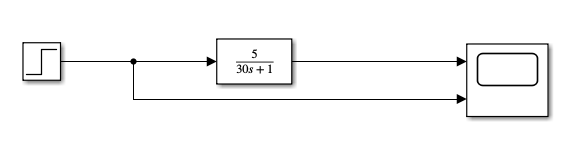
\includegraphics[width=0.7\textwidth]{EXERCICE 6 1.png}
\end{center}\textsf{\textbf{Graph avec grille :}}
\begin{center}
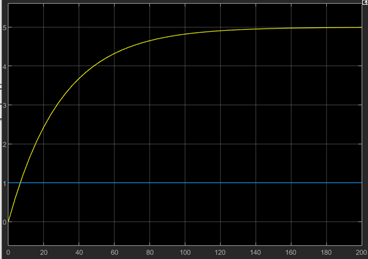
\includegraphics[width=0.7\textwidth]{EXERCICE 6 2.png}
\newpage
\end{center}\textsf{\textbf{Système en Boucle Fermée :}}
\begin{center}
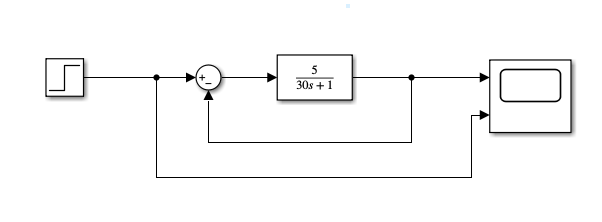
\includegraphics[width=0.7\textwidth]{EXERCICE 6 3.png}
\end{center}\textsf{\textbf{Graph avec grille :}}
\begin{center}
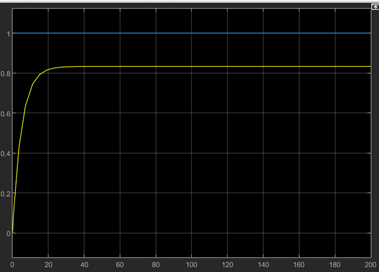
\includegraphics[width=0.7\textwidth]{EXERCICE 6 4.png}
\end{center}
\newpage

\textsf{\textbf{Exercice 7 :}}
\begin{problem}{Étude d’un circuit RC soumis à un échelon}{exercise-label-7}
Soit le circuit RC suivant attaqué par un échelon d’amplitude \( 24\,\text{V} \), avec \( R = 50\,\Omega \) et \( C = 100\,\mu\text{F} \). Le condensateur est initialement déchargé.

\begin{center}
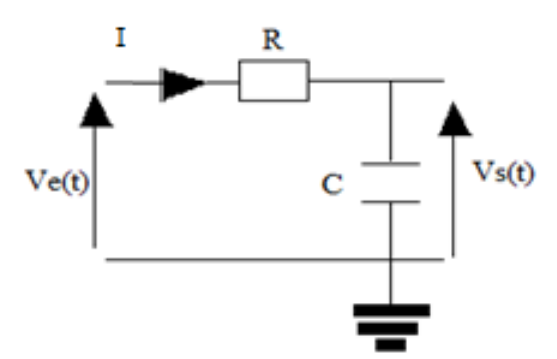
\includegraphics[width=0.7\textwidth]{exercice7.png}
\end{center}

\begin{enumerate}
    \item \textbf{Modélisation Simulink:} Établissez le modèle Simulink de ce montage.
    \item \textbf{Visualisation des courbes:} Visualisez les courbes en fonction du temps, de la tension, et du courant obtenus au niveau du condensateur.
    \item \textbf{Analyse théorique:} Établissez l’étude théorique et interprétez les résultats obtenus.
\end{enumerate}
\end{problem}

\textsf{\textbf{Solution :}}

\begin{center}
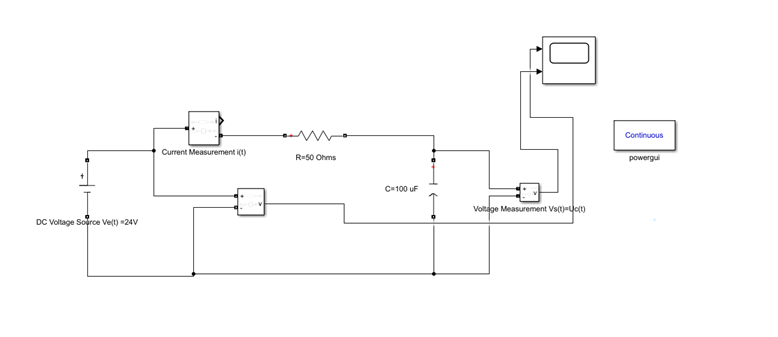
\includegraphics[width=1\textwidth]{EXERCICE 7 1.png}
\end{center}
\begin{center}
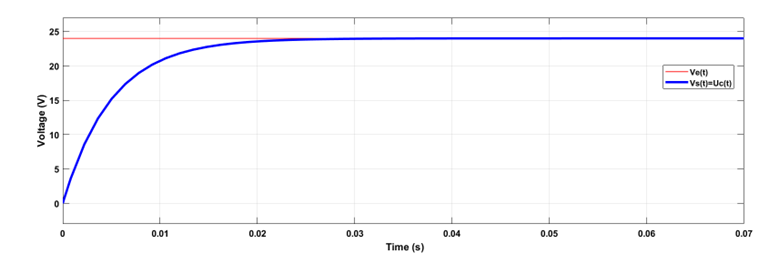
\includegraphics[width=1\textwidth]{EXERCICE 7 2.png}


\bibliographystyle{apalike}
\bibliography{references}

\end{document}
